\subsection{Chapter 22 - Electromagnetic induction}

\subsubsection{Overview}\label{chapter:induction}

In this chapter, we introduce the tools to model the connection between the magnetic and the electric field. In particular, we will see how a changing magnetic field can be used to induce an electric current, which is the basic principle behind the electric generators that power our life. We will also briefly discuss how electromagnetic waves are formed.

\begin{framed}
\textbf{Learning Objectives}\\
\begin{itemize}
\item Understand how to apply Faraday's law to determine an induced voltage.
\item Understand how to model the induced voltage in a moving conductor.
\item Understand how to model an electric generator.
\item Understand how electromagnetic induction affects electric motors.
\item Understand how to model electric transformers.
\item Understand how electromagnetic waves are formed.
\end{itemize}
\end{framed}

\begin{framed}
\textbf{Think About It}\\
How does one make electricity with a hydroelectric dam?

\begin{enumerate}
\item By running water through a coil to induce a current.
\item By using water to rotate a coil inside of a fixed magnetic field.
\item By using water to charge a metallic surface by friction, and then maintaining that potential difference.
\end{enumerate}

\begin{framed}
\textbf{Answer}\\
\begin{enumerate}[resume]
\item
\end{enumerate}
\end{framed}
\end{framed}

\subsubsection{Faraday's Law}

In the previous chapter, we described how an electric current produces a magnetic field. In this chapter, we describe how an electric current can be produced (or rather, ``induced'') by a magnetic field. The most important aspect of electromagnetic induction is that it always involves quantities that change with time. In past chapters, we have only dealt with static electric and magnetic fields, static charges (for electric fields), and static currents (for magnetic fields).

Faraday's law connects the flux of a \textbf{time-varying} magnetic field to an induced voltage (rather than a current). For historical reasons, the induced voltage is also called an induced ``electromotive force'' (emf), even if it is a voltage and not a force. Faraday's law is as follows:
\begin{equation}
\boxed{\Delta V = -\frac{d\Phi_B}{dt}}
\end{equation}
where $\Delta V$ is the induced voltage, and  $\Phi_B$ is the flux of the magnetic field through an open surface, defined in the same way as the flux of the electric field (Section~\ref{sec:gauss:flux}):
\begin{equation}
\Phi_B = \int_S \vec B\cdot d\vec A
\end{equation}
If the magnetic field has a constant magnitude over the surface, $S$, and always makes the same angle with the surface, then the flux can be written as:
\begin{equation}
\Phi_B =  \vec B\cdot\vec A
\end{equation}
where the magnitude of the vector $\vec A$ is equal to the area of the surface, and the vector $\vec A$ is normal to the surface.

The surface, $S$, is defined by a closed path. The induced voltage can be thought of as an ideal battery placed in the closed path that defines the surface (right-hand panel of Figure~\ref{fig:induction:faraday}). The minus sign in Faraday's Law indicates the direction of the current associated with the induced voltage. It is important to note that an induced voltage only exists if the flux of the magnetic field changes (since the induced voltage is given by the time-derivative of the flux). Remember, induction is all about time-varying fields! This is better illustrated with an example.

Consider a loop of wire that is immersed in a uniform magnetic field, $\vec B$, that is perpendicular to the plane of the loop, as illustrated in Figure~\ref{fig:induction:faraday}. As time goes by, the magnetic field increases in strength, as shown in going from the left panel to the right panel. The flux of the magnetic field through the loop increases in magnitude, and a voltage is thus induced across the wire (illustrated by the ideal battery on the loop in the right panel), leading to an induced current, $I$.

\begin{figure}[!htbp]
\centering
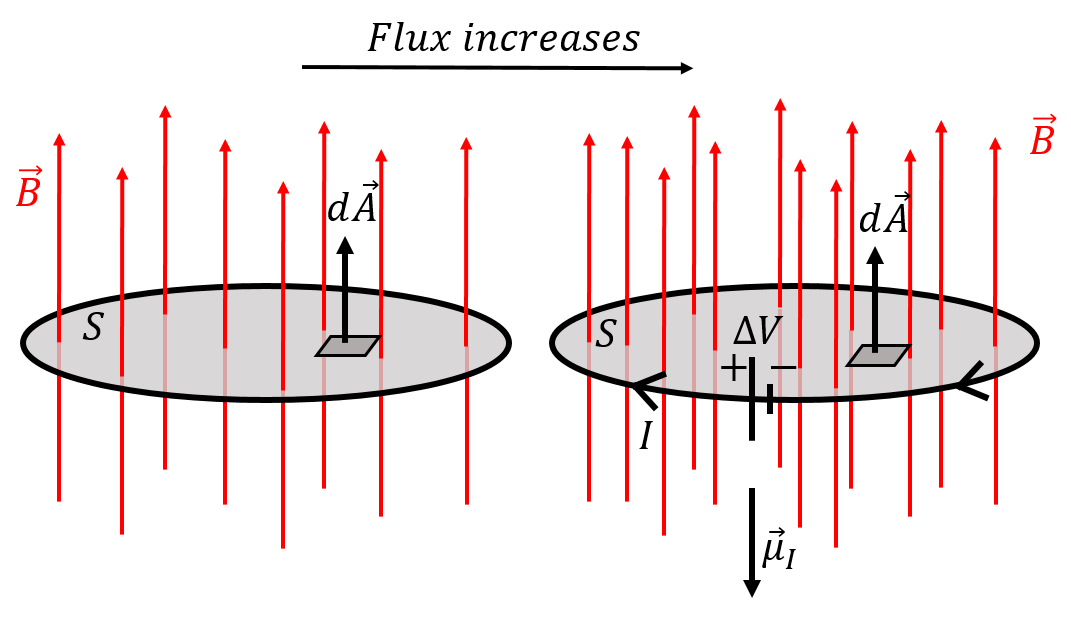
\includegraphics[width=0.6\linewidth]{files/faraday-e5e8ce9b9d57169da249773be45edc7c.png}
\caption[]{As the magnetic field increases, so does the flux through the loop that is shown. The changing flux results in an induced voltage, which produces an induced current that has a magnetic moment, $\vec \mu_I$. The induced current produces a magnetic field in a direction to oppose the changing flux.}
\label{fig:induction:faraday}
\end{figure}

When calculating the flux of the magnetic field, we have to choose the surface element vector, $d\vec A$, to be perpendicular to the surface over which we calculate the flux. There are two choices\footnote{Recall that this ambiguity is resolved when using Gauss' Law by always choosing $d\vec A$ to point ``outwards'', which only makes sense when the surface is closed. With an open surface, there is no inside or outside, and we are left with the ambiguity.} (upwards or downwards, referring to Figure~\ref{fig:induction:faraday}); we \textbf{chose} to define $d\vec A$ to point upwards. Thus, the magnetic flux is positive in both panels, and increases with time. The derivative, $d\vec B/dt$, is positive and the right-hand side of Faraday's equation is negative because of the negative sign in front. Had we chosen to define $d\vec A$ to point downwards, the right-hand side of Faraday's law would be negative.

We can describe the direction of the induced current, $I$, in terms of its magnetic dipole moment (Section~\ref{sec:MagneticForce:dipolemoment}), $\vec\mu_I$, also shown in Figure~\ref{fig:induction:faraday}. The overall sign on the right-hand side of Faraday's law is determined by our (arbitrary) choice of the direction $d\vec A$. With this choice, we found that the right-hand side of Faraday's law is negative:
\begin{equation}
\Delta V = -\frac{d\Phi_B}{dt}=\text{a negative number}
\end{equation}
\textbf{The overall sign of $\Delta V$ indicates whether the magnetic moment of the induced current is parallel ($\Delta V$ positive) or anti-parallel ($\Delta V$ negative) to $d\vec A$}. This allows us to determine the direction of the induced current, and thus the direction of the ideal battery that represents the induced voltage. In general, when possible, it is common to choose the direction of $d\vec A$ to be parallel to the magnetic field vector, so that the flux is positive (although this does not guarantee that its derivative is positive).

\paragraph{Lenz's law}

The minus sign in Faraday's law is sometimes called ``Lenz's law'', and ultimately comes from the conservation of energy. In Figure~\ref{fig:induction:faraday} above, we found that as the magnetic flux increases through the loop, a current is induced. That \textbf{induced current will also produce a magnetic field} (in the direction of its magnetic dipole moment vector, $\vec \mu_I$).

Lenz's law states that the ``induced current will always be such that the magnetic field that it produces counteracts the changing magnetic field that induced the current''. In Figure~\ref{fig:induction:faraday}, the magnetic field points in the upwards direction, and increases in magnitude with time. The induced current produces a magnetic field that points downwards to counteract the changing magnetic field, and preserve a constant flux through the loop. If this were not the case, the induced current would be in the opposite direction, contributing to the increasing magnetic flux through the loop, inducing more current, producing more flux, inducing more current, etc. Clearly, this would lead to an infinite current and solve the world's energy crisis. Unfortunately, conservation of energy (expressed here as Lenz's law) prevents this from happening.

You can use Lenz's law to determine the direction of induced currents. In general:

\begin{itemize}
\item If the magnitude of the magnetic \textbf{flux is increasing} in the loop, then the induced current produces a magnetic field that is in the \textbf{opposite direction} from the original magnetic field.
\item If the magnitude of the magnetic \textbf{flux is decreasing} in the loop, then the induced current produces a magnetic field that is in the \textbf{same direction} as the original magnetic field.
\end{itemize}

The negative sign in Faraday's law is not arbitrary (as we saw above, it gives the correct direction for the magnetic moment of the induced current, given our arbitrary choice of direction for $d\vec A$). In practice, one can often use Lenz's law to determine the direction of the induced current (so that it counteracts the changing flux), and Faraday's law to determine the magnitude of the induced voltage.

\begin{framed}
\textbf{Checkpoint}\\
A loop of wire is immersed in a constant and uniform magnetic field out of the page, perpendicular to the plane of the loop, as shown in Figure~\ref{fig:induction:areaup}. If the radius of the loop increases with time, in which direction will be the current induced in the loop?

\begin{figure}[!htbp]
\centering
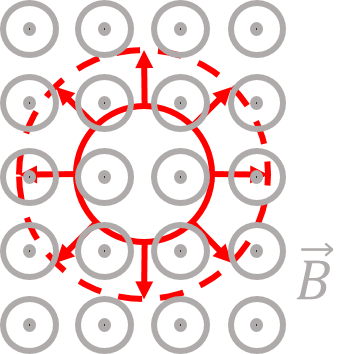
\includegraphics[width=0.2\linewidth]{files/areaup-dd85169b19d9857148685da749c5d617.png}
\caption[]{A loop whose radius increases with time.}
\label{fig:induction:areaup}
\end{figure}

\begin{enumerate}
\item Since the magnetic field is constant, there is no induced current.
\item Clockwise.
\item Counter-clockwise.
\end{enumerate}

\begin{framed}
\textbf{Answer}\\
\begin{enumerate}[resume]
\item
\end{enumerate}
\end{framed}
\end{framed}

\begin{framed}
\textbf{Checkpoint}\\
A loop of wire is immersed in a constant and uniform magnetic field out of the page, perpendicular to the plane of the loop, as shown in Figure~\ref{fig:induction:loopout}. If the loop is pulled out of the region of magnetic field, as shown, in which direction is the induced current in the loop?

\begin{figure}[!htbp]
\centering
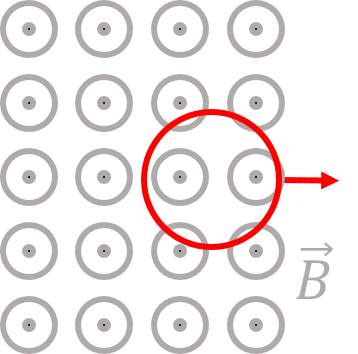
\includegraphics[width=0.2\linewidth]{files/loopout-c0263da4236539f3c5aaa3e78bcf7ece.png}
\caption[]{A loop being pulled out of a region with uniform magnetic field.}
\label{fig:induction:loopout}
\end{figure}

\begin{enumerate}
\item Since the magnetic field is constant, there is no induced current.
\item Clockwise.
\item Counter-clockwise.
\end{enumerate}

\begin{framed}
\textbf{Answer}\\
\begin{enumerate}[resume]
\item
\end{enumerate}
\end{framed}
\end{framed}

\begin{framed}
\textbf{Example 22.1}\\
A uniform time-varying magnetic field is given by:
\begin{equation}
\vec B(t) = B_0(1+at)\hat z
\end{equation}
where $B_0$ and $a$ are positive constants. A coil, made of $N$ circular loops of radius, $r$, lies in the $x -y$ plane. If the coil has a total resistance, $R$, what is the magnitude and direction of the current induced in the coil?

\begin{framed}
\textbf{Solution}\\
The coil is made of $N$ loops of wire. Each loop of wire can be treated independently, and each will have its own induced voltage across it. Since each loop is the same, they will all have the same induced voltage, and the total voltage induced across the coil, $\Delta V$, will be given by:
\begin{equation}
\Delta V = -N \frac{d\Phi_B}{dt}
\end{equation}
where $\Phi_B$ is the flux through any one of the loops. That is, each loop is similar to an ideal battery, and the coil is similar to placing all of these batteries in series, so that the voltages from each battery sum together.

The coil lies the $x -y$ plane, perpendicular to the increasing magnetic field, similar to the situation depicted in Figure~\ref{fig:induction:faraday}. Since the magnetic field is uniform over the surface of the coil, we do not need an integral to determine the flux. We define the area vector, $\vec A$, to be in the positive $z$ direction (parallel to the magnetic field):
\begin{equation}
\vec A = A \hat z = \pi r^2 \hat z
\end{equation}
The flux through one circular loop of radius, $r$, is given by:
\begin{equation}
\Phi_B (t) &= \vec B \cdot \vec A = ( B_0(1+at)\hat z) \cdot (\pi r^2 \hat z) =B_0(1+at) (\pi r^2)
\end{equation}
We can apply Faraday's law to determine the induced voltage:
\begin{equation}
\Delta V &= -N \frac{d\Phi_B}{dt} = -N \frac{d}{dt} B_0(1+at) (\pi r^2)\\
&=-NB_0a\pi r^2
\end{equation}
Since the induced voltage is negative, the magnetic moment of the induced current points in the negative $z$ direction (opposite to our choice of direction for $\vec A$). This is consistent with Lenz's law, since the magnetic field increases in the positive $z$ direction, the induced current will produce a magnetic field in the negative $z$ direction to counteract the changing flux. The magnitude of the induced current is given by Ohm's Law:
\begin{equation}
I = \frac{\Delta V}{R}=\frac{NB_0a\pi r^2}{R}
\end{equation}

\textbf{Discussion:} In this example, we determined the induced voltage and current in a coil made of $N$ identical loops. We argued that one can sum the induced voltages from the $N$ loops, as these can be thought of as ideal batteries in series. We found that the direction of the induced current as obtained from Faraday's law was consistent with the expectation from Lenz's law.
\end{framed}
\end{framed}

\begin{framed}
\textbf{Olivia's Thoughts}\\
Here are some steps you can follow to find the direction of the current using Lenz's law.

\begin{enumerate}
\item Draw a diagram showing the loop/coil and the magnetic field lines.
\item I like to indicate whether the flux is increasing or decreasing by drawing a ``flux arrow'' (a term that I made up, so please don't use it around physicists because they won't know what you're talking about). If the flux is increasing, this will point in the same direction as the field lines. If it is decreasing, the flux arrow will point opposite to the field lines.
\item Assume that the induced current is in the clockwise direction and use the axial right hand rule to determine the direction of the induced magnetic field.
\item Repeat Step 2 assuming the counter-clockwise direction.
\item Decide which direction for the induced current will give you the desired field. We want the induced field to point opposite to the flux arrow.
\end{enumerate}

This is how you would apply this method to Example~22.1 (note that I am using the example of a loop instead of a coil but the idea is the same):

\begin{enumerate}
\item We draw the diagram, as in Figure~\ref{fig:induction:lenzs_example}a.
\item To show that the flux is increasing, I have drawn a ``flux arrow'' (again, made up) in the direction of the field lines (the $+z$ direction).
\item If the current is clockwise, the induced field points in the $-z$ direction inside the loop (Figure~\ref{fig:induction:lenzs_example}b).
\item If the current is counter-clockwise, the induced field points in the $+z$ direction inside the loop (Figure~\ref{fig:induction:lenzs_example}c).
\item Since the flux is increasing, we want an induced current that will decrease the flux. We choose the clockwise current because the induced field points opposite to the flux arrow.
\end{enumerate}

\begin{figure}[!htbp]
\centering
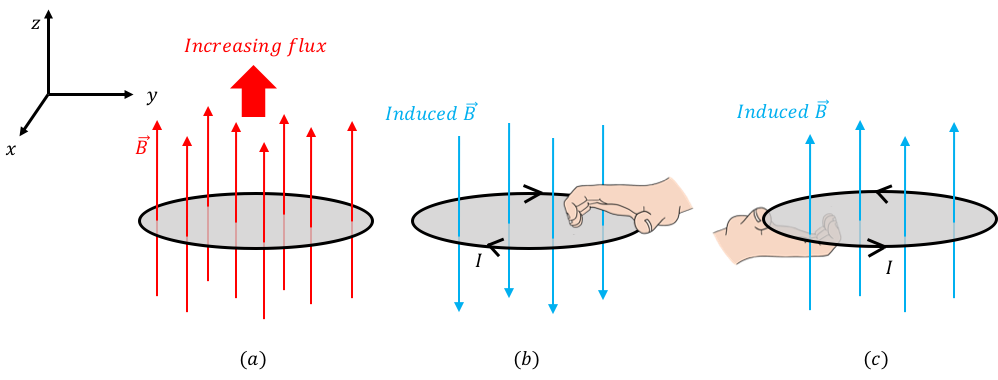
\includegraphics[width=0.9\linewidth]{files/lenzs_example-d7f248103d55bc911f37a92a8fc83217.png}
\caption[]{(a) An increasing magnetic field through a loop. (b) A clockwise current induces a magnetic field in the $-z$ direction. (c) A counter-clockwise current induces a magnetic field in the $+z$ direction.}
\label{fig:induction:lenzs_example}
\end{figure}
\end{framed}

\subsubsection{Induction in a moving conductor}

If we define a loop of wire, there are two ways in which the magnetic flux through that loop can change:

\begin{enumerate}
\item The magnetic field can change magnitude or direction, as we saw in Example~22.1.
\item The loop can change size or orientation relative to the magnetic field.
\end{enumerate}

In this section, we examine the latter case, sometimes called ``motional emf'', as the induced voltage is the result of motion from the loop in which the voltage is induced.

\paragraph{Motion of a bar on two parallel rails}

Consider a U-shaped rail in a uniform magnetic field on top of which a bar can slide with no friction, as illustrated in Figure~\ref{fig:induction:rail}. The bar of length $L$ moves to the right with a constant speed, $v$.

\begin{figure}[!htbp]
\centering
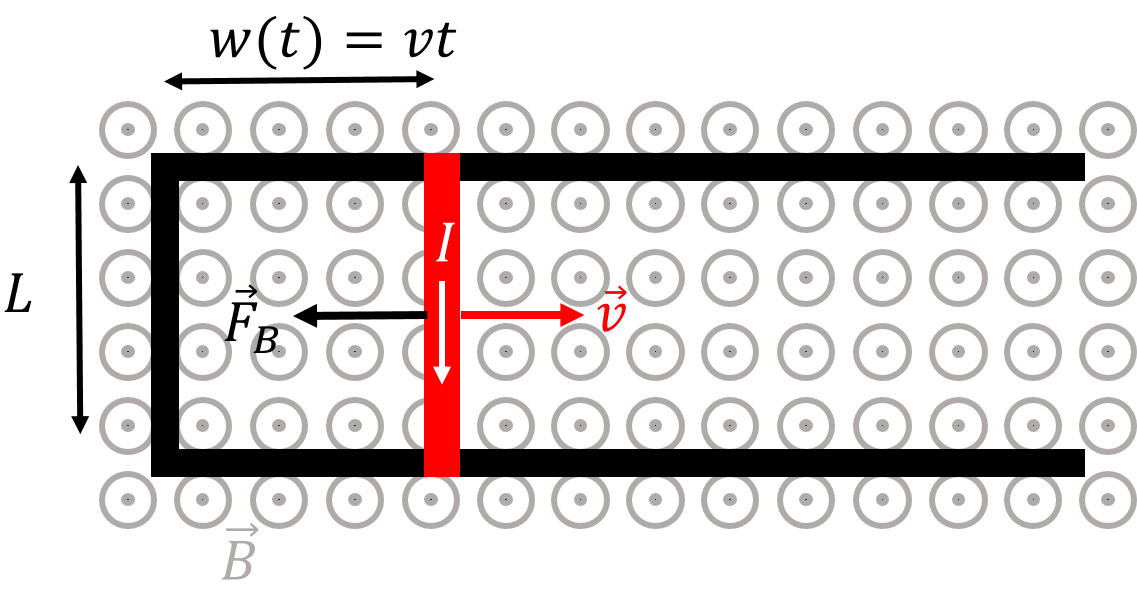
\includegraphics[width=0.6\linewidth]{files/rail-8a3f3d543097c528778d803819acd89a.png}
\caption[]{A U-shaped rail on top of which a bar of length, $L$, can slide. The system is immersed in a magnetic field that points out of the page. The bar moves to the right with a constant speed, $v$.}
\label{fig:induction:rail}
\end{figure}

The bar and the rails form a closed loop of area:
\begin{equation}
A(t)=Lw(t)=Lvt
\end{equation}
that increases with time. The magnitude of the flux through the loop will increase with time, resulting in an induced current (clockwise, according to Lenz's law). At some time $t$, the flux through the loop is given by:
\begin{equation}
\Phi_B (t) &=  \vec B \cdot \vec A =BA=BLvt
\end{equation}
where we chose $\vec A$ to be parallel to the magnetic field vector.

Since we already used Lenz's law to argue that the current must be in the clockwise direction, we can use Faraday's law to determine the magnitude of the induced voltage and ignore the negative sign:
\begin{equation}
\Delta V = \frac{d \Phi_B}{dt}=\frac{d}{dt}BLvt = BLv
\end{equation}

Suppose that the rails are superconducting (have no resistance), and that the bar has a resistance, $R$. The current through the loop is then given by Ohm's Law:
\begin{equation}
I=\frac{\Delta V}{R}=\frac{BLv}{R}
\end{equation}
As the current moves through the bar, it will heat up the bar by dissipating energy at a rate of:
\begin{equation}
P=I^2 R = \frac{B^2L^2v^2}{R}
\end{equation}
Thus, the bar cannot possibly move at a constant speed on its own, or energy would be produced out of nothing. There must be a force exerted on the bar to keep it moving at constant speed.

Recall that a current-carrying wire in a magnetic field will experience a force from the magnetic field. In this case, the bar of length $L$ carries a current, $I$, in a magnetic field, $\vec B$ (perpendicular to the current), so that the force exerted on the bar is given by:
\begin{equation}
\vec F_B = I \vec L \times \vec B
\end{equation}
and points to the left (right-hand rule). The magnitude of the force is given by:
\begin{equation}
F_B = ILB = \frac{B^2L^2v}{R}
\end{equation}
Thus, in order for the bar to move at constant velocity towards the right, a force with the same magnitude must be exerted towards the right. In other words, work must be done to pull the bar to the right, by exerting a force with the magnitude, $F_B$. The rate at which that work must be done is given by:
\begin{equation}
P &= \frac{d}{dt}W\\
&=\frac{d}{dt}\vec F \cdot dx\\
&=\vec F\cdot \frac{dx}{dt}\\
&=\vec F\cdot \vec v = Fv\\
&=\frac{B^2L^2v^2}{R}
\end{equation}
where we assumed that the bar moves in the positive $x$ direction. This is exactly the rate at which electric energy is dissipated in the bar! In other words, by doing mechanical work on the bar, we can create an induced current that will dissipate that energy at the same rate at which we do work. We can convert mechanical work into electrical energy!

\begin{framed}
\textbf{Olivia's Thoughts}\\
I'll quickly sum up what is happening in this example:

\begin{enumerate}
\item We pull the bar to the right.
\item The flux in the loop increases, which produces a current in the clockwise direction according to Lenz's law. We can calculate the potential difference to produce this current using Faraday's law.
\item The downwards current in the bar produces a force to the left according to the Lorentz force, $F=I\vec{l}\times \vec{B}$. To move the bar at a constant velocity, the force we apply to pull the bar should be equal to the Lorentz force.
\item Assuming the bar has a resistance, power is dissipated in the resistor. Power is dissipated at the same rate as the work done by us to pull the bar.
\end{enumerate}
\end{framed}

Finally, also note that this situation is closely related to the Hall effect, which is simply a different way to think about this problem. Consider the electrons that are in the bar, as the bar moves at constant speed to the right through the magnetic field (ignore the existence of the U-shaped rail). The electrons will experience a magnetic force that is upwards (consistent with the direction of the induced current discussed above). Eventually, electrons accumulate at the top of the bar, and start preventing more electrons from accumulating there, by producing an electric field, $\vec E$, in the bar. The equilibrium condition is that the magnetic force and the electric force have the same magnitude (and opposite directions):
\begin{equation}
qvB &= qE\\
E &= vB
\end{equation}
The (Hall) potential difference, across the bar of length, $L$, with an electric field, $E$, is given by:
\begin{equation}
\Delta V_{Hall} = EL = vBL
\end{equation}
where we assumed that the electric field is uniform in the bar. This potential difference is identical to the one that we calculated from Faraday's law. Viewing this example as a different manifestation of the Hall effect provides some insight into what is actually happening at the microscopic level when a current is induced.

\paragraph{The generator}

An electrical generator is used to create an alternating induced voltage/current by rotating a coil inside of a constant and uniform magnetic field. In this case, the current is induced because the angle between the magnetic field and the surface element vector $d\vec A$ changes with time.

Consider a single loop of wire with area $A$ that can rotate in a uniform and constant magnetic field, $\vec B$, as illustrated in Figure~\ref{fig:induction:generator}.

\begin{figure}[!htbp]
\centering
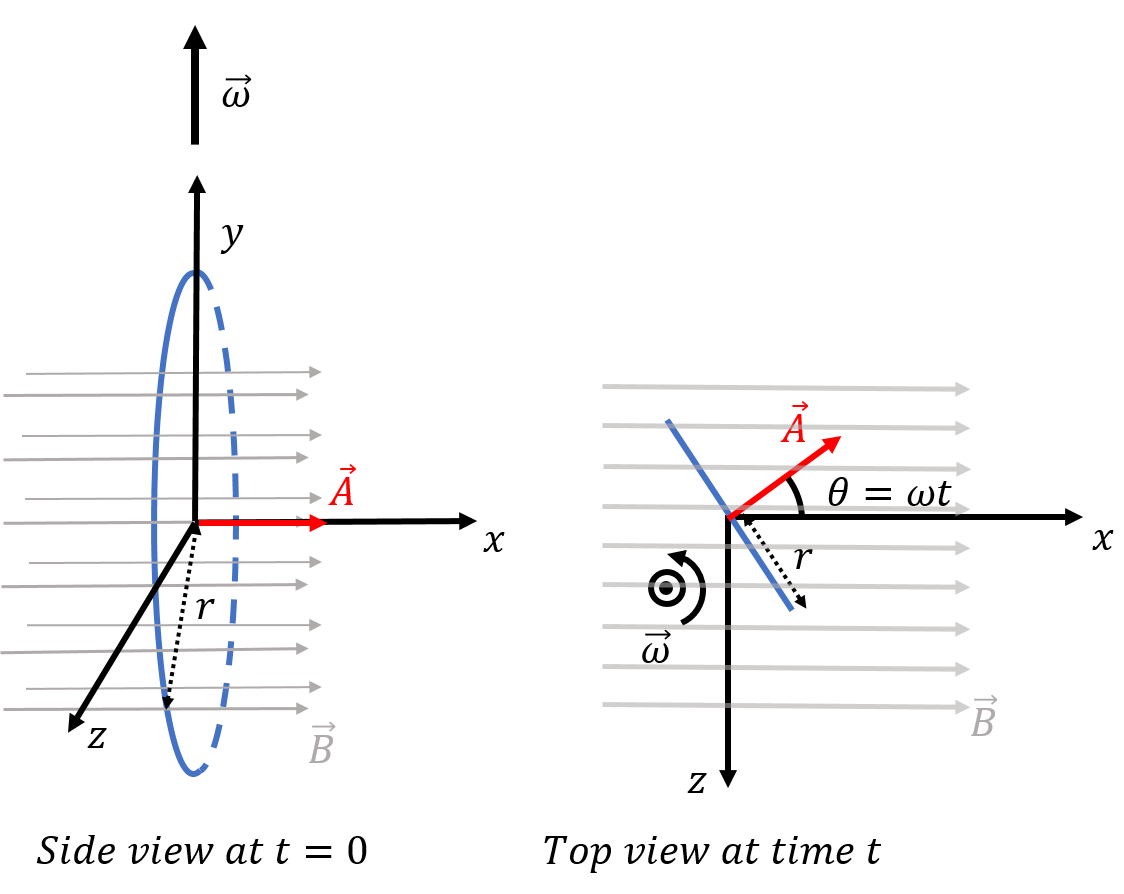
\includegraphics[width=0.6\linewidth]{files/generator-d90ce872c1eb265a4b57a78c94dce269.png}
\caption[]{A loop of wire rotates in a constant and uniform magnetic field. At time $t=0$ (left panel), the loop lies in the $yz$ plane. The loop rotates about the $y$ axis, with a constant angular velocity, $\vec \omega$. At some time $t$ later, the loop has rotated through an angle $\theta = \omega t$ (right panel, as seen from above, looking down on the $xz$ plane).}
\label{fig:induction:generator}
\end{figure}

Referring to the coordinate system that is illustrated in Figure~\ref{fig:induction:generator}, the loop has a constant angular velocity, $\vec\omega$, in the positive $y$ direction and rotates about the $y$ axis (with the origin at the centre of the coil). At time $t=0$ (left panel), the loop lies in the $yz$ plane, and we choose the vector $\vec A$ (used to calculate the flux) to be in the positive $x$ direction at time $t=0$. As the coil rotates, so will the vector $\vec A$, which is easier to visualize than the coil. At some time $t$, the vector $\vec A$ will make an angle $\theta=\omega t$ with the $x$ axis (right panel). The magnetic field is constant and in the positive $x$ direction, $\vec B = B\hat x$. That is, the angle between the vector $\vec A$ and the magnetic field, $\vec B$, will be given by $\theta = \omega t$.

At some time, $t$, the vector $\vec A$ is given by:
\begin{equation}
\vec A(t) = A(\cos\theta \hat x -\sin\theta \hat z) = A(\cos(\omega t) \hat x -\sin(\omega t)\hat z)
\end{equation}

We can calculate the flux of the magnetic field through the loop at some time $t$:
\begin{equation}
\Phi_B(t) =  \vec B \cdot \vec A = (B\hat x) \cdot (A\cos(\omega t) \hat x -A\sin(\omega t)\hat z)=AB\cos(\omega t)
\end{equation}
where we did not use the integral for the flux, since the magnetic field is constant over the area of the loop. The induced voltage is given by Faraday's law:
\begin{equation}
\Delta V = - \frac{d\Phi_B}{dt}  =  - \frac{d}{dt}AB\cos(\omega t) =  AB\omega\sin(\omega t)
\end{equation}
If the generator includes $N$ loops in a coil, then the induced voltage is given by:
\begin{equation}
\Delta V = NAB\omega\sin(\omega t)
\end{equation}
As you can see, the voltage oscillates with time, between $\pm NAB\omega$, corresponding to alternating voltage. Furthermore, since the sign of $\Delta V$ changes with time (due to the sine function), the relative orientation between $\vec A$ and the magnetic dipole moment of the induced current, also changes with time, indicating that the induced current in the coil changes direction every half-turn (alternating current).

The generators that produce the alternating voltages that we find in our outlets work on the same principle. For example, in a hydro-electric dam, the water pressure from the height of the dam is used to force water through a turbine (essentially a propeller) that rotates a set of coils inside of a strong permanent magnet. Various controls allow the rotational frequency of the turbine to be adjusted in order to produce alternating current of the desired frequency ($50 {\rm Hz}$ in most of the world, $60 {\rm Hz}$ in North America and a few other countries).

Since the generator produces current that can dissipate electrical energy, one has to do work in order to keep the coil in the generator rotating. As the coil rotates, a current is induced in the coil. A current in a circular loop that is immersed in a magnetic field will experience a torque, $\vec \tau$, given by:
\begin{equation}
\vec \tau = \vec \mu \times \vec B
\end{equation}
where $\vec \mu$ is the magnetic dipole moment of the coil with induced current, $I$. If the current from the coil dissipates its energy in a system with resistance, $R$, then the current in the coil is given by Ohm's Law:
\begin{equation}
I = \frac{\Delta V}{R}=\frac{NAB\omega\sin(\omega t)}{R}
\end{equation}
The magnetic moment, $\vec \mu$, for the current in the coil is given by:
\begin{equation}
\vec \mu &= I\vec A = \frac{NAB\omega\sin(\omega t)}{R} (A(\cos(\omega t) \hat x -\sin(\omega t)\hat z))\\
&=\frac{NA^2B\omega\sin(\omega t)}{R} (\cos(\omega t) \hat x -\sin(\omega t)\hat z)
\end{equation}
The torque exerted by the magnetic field on the coil with the induced current is thus given by:
\begin{equation}
\vec \tau &= \vec \mu \times \vec B = \left(\frac{NA^2B\omega\sin(\omega t)}{R} (\cos(\omega t) \hat x -\sin(\omega t)\hat z)\right) \times (B\hat x)\\
&=\frac{NA^2B^2\omega\sin(\omega t)}{R}(\cos\omega(t)(\hat x \times \hat x)-\sin(\omega t)(\hat z \times \hat x))\\
&=-\frac{NA^2B^2\omega\sin^2(\omega t)}{R}\hat y
\end{equation}
Note that the torque exerted on the loop is always in the negative $y$ direction, as every term in the torque is either strictly positive ($N,R$) or squared ($\sin^2(\omega t)$). The torque exerted by the magnetic field on the coil is thus always in the opposite direction of rotation (recall that the coil has an angular velocity in the positive $y$ direction). This is sometimes called ``counter torque''. If we want the coil to maintain a constant angular velocity, then we must exert a torque in the positive $y$ direction to counter the torque from the magnetic field. Note that the torque that we must exert to keep the coil rotating with constant angular velocity is not constant in time (but always in the same direction).

You can easily verify that the work that you must do by exerting the torque is the same as the electrical power dissipated by the current in the resistor, $R$. The generator is thus a device to convert mechanical work into electrical energy (with AC current, in particular).

\subsubsection{Back EMF in an electric motor}

There are many similarities between electric motors and generators, and in fact, they can be thought of as the same device. In an electric motor, current is passed through a coil in a magnetic field, so that a torque is exerted on the coil, and it starts to rotate. In a generator, one exerts a torque to rotate the coil, thus inducing a current.

Consider an electric motor. As we supply current to the motor, the coil starts to rotate. But, a rotating coil in a magnetic field results in an induced current. By Lenz's law, the induced current in the coil of a motor has to be in the direction opposite to the current that we put in, since otherwise, the motor would start to spin infinitely fast. We call this effect ``back emf'', as the motor effectively acts like a battery that opposes current, as illustrated in Figure~\ref{fig:induction:backemf}

\begin{figure}[!htbp]
\centering
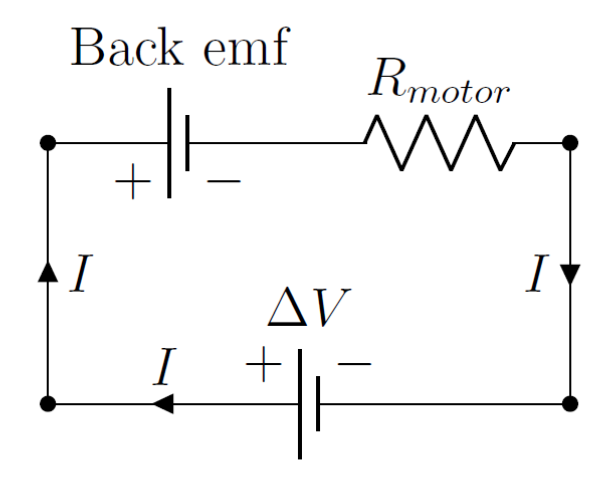
\includegraphics[width=0.3\linewidth]{files/backemf-884fc6af7b406bccea4cff3c4f67981b.png}
\caption[]{A simple circuit illustrating how a motor, with resistance, $R_{motor}$, will generate a ``back emf'', equivalent to a battery that produces a voltage in the direction to oppose the current from the actual battery that is powering the motor, $\Delta V$.}
\label{fig:induction:backemf}
\end{figure}

If you connect an electric motor to a voltage source, initially, the motor is at rest, so there will be no back emf and the current through the circuit will be very large (motors have a small resistance, so that the electrical energy is converted into work rather than heating up the motor). As the motor starts to spin faster, the back emf from the motor grows, reducing the current in the circuit. If there is no load on the motor (i.e. the motor can rotate freely with no friction), then the rotational speed of the motor will increase until the back emf exactly matches the voltage supplied to the motor. The motor will then rotate at constant speed, with (almost) no current in the circuit (if the motor slows down, the emf will decrease, and the current will increase to speed up the motor). If there is a load on the motor (because it's making something turn), then the motor will rotate at a speed that is lower than that which would result in zero current, since some of that current is now used by the motor to exert a torque.

You may notice that the lights in your house dim briefly as your refrigerator turns on. This is because your refrigerator uses an electric motor that initially draws a large current when it turns on, large enough to produce a voltage drop in the circuit of your house to observe a dimming of your lights. You may also notice that if you plug the inlet or outlet of a hair dryer, the hair dryer turns off quickly. In this case, by blocking the flow of air, you prevent the motor in the hair dryer from rotating; this results in a large current through its coil, since there is no back emf. Most hair dryers have a circuit breaker that will detect this large current and open the circuit to prevent the coil in the motor from over heating and melting. In general, one should not prevent an electric motor from rotating, as this will result in a large current through the motor that could melt its internal components.

\subsubsection{The induced electric field and eddy currents}

So far, we have described electromagnetic induction in terms of the voltage that is induced by a changing magnetic field. This voltage is related to an electric field, which we discuss in this section. In Faraday's  Law, the voltage is induced across a closed loop (and can be thought of as an ideal battery placed in the loop). This is illustrated in Figure~\ref{fig:induction:inducedE} which shows a loop in the plane of the page, and a magnetic field out of the plane of the page.

\begin{figure}[!htbp]
\centering
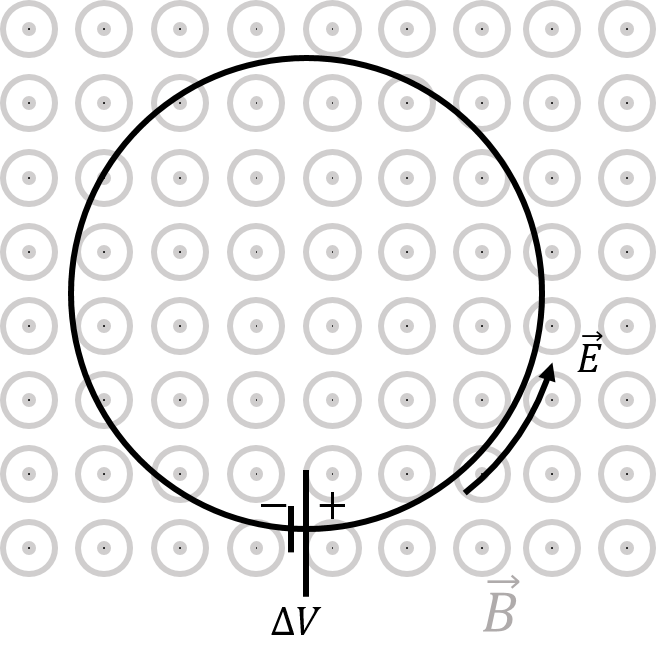
\includegraphics[width=0.4\linewidth]{files/inducedE-7bdece303343897b313b1edc5e6f97b8.png}
\caption[]{A varying magnetic field will induce a circular electric field.}
\label{fig:induction:inducedE}
\end{figure}

\begin{framed}
\textbf{Checkpoint}\\
In Figure~\ref{fig:induction:inducedE}, in order to produce the induced voltage as shown, is the magnetic field increasing or decreasing?

\begin{enumerate}
\item The magnetic field is increasing.
\item The magnetic field is decreasing.
\end{enumerate}

\begin{framed}
\textbf{Answer}\\
\begin{enumerate}[resume]
\item
\end{enumerate}
\end{framed}
\end{framed}

As you recall, the electric potential difference between two points, $A$ and $B$, is obtained from the electric field:
\begin{equation}
\Delta V = \int_A^B \vec E\cdot d\vec l
\end{equation}
In the case of an induced voltage across a loop, the points $A$ and $B$ are the same. The integral is thus over a closed path:
\begin{equation}
\Delta V = \oint \vec E\cdot d\vec l
\end{equation}
We can include this into Faraday's law by using the electric field instead of the potential difference:
\begin{equation}
\Delta V =-\frac{d\Phi_B}{dt}\\
\end{equation}
\begin{equation}
\therefore \;\;\boxed{\oint \vec E\cdot d\vec l = -\frac{d\Phi_B}{dt}}
\end{equation}
where the last line is a more general form of Faraday's law. Note that in the case of electrostatics, where the electric field is produced by a distribution of charges, the integral $\oint \vec E\cdot d\vec l$ must be zero, since the electric force is conservative; the work done by the electric field on a charge $q$ over a closed path, which is just a charge $q$ multiplied by that integral, must be zero. The force from an electric field that is induced by a time-varying magnetic field is not conservative!

Faraday's law as expressed with the electric field is much more general, and implies that a time-varying magnetic field will induce an electric field. This is true, independently of there existing a physical wire to carry the induced current.

\begin{framed}
\textbf{Example 22.2}\\
A circular region with radius $R$ contains a magnetic field that is uniform, and decreasing in magnitude with time:
\begin{equation}
\vec B(t) = B_0(1-at)\hat z
\end{equation}
where $a$ and $B_0$ are positive constants. Determine the electric field at a distance, $r$, from the centre of the region, inside and outside of the region with the magnetic field.

\begin{framed}
\textbf{Solution}\\
Figure~\ref{fig:induction:inducedE2} shows the circular region of magnetic field, as well as a circular path of radius $r$ that defines the region over which we calculate the flux of the magnetic field.

\begin{figure}[!htbp]
\centering
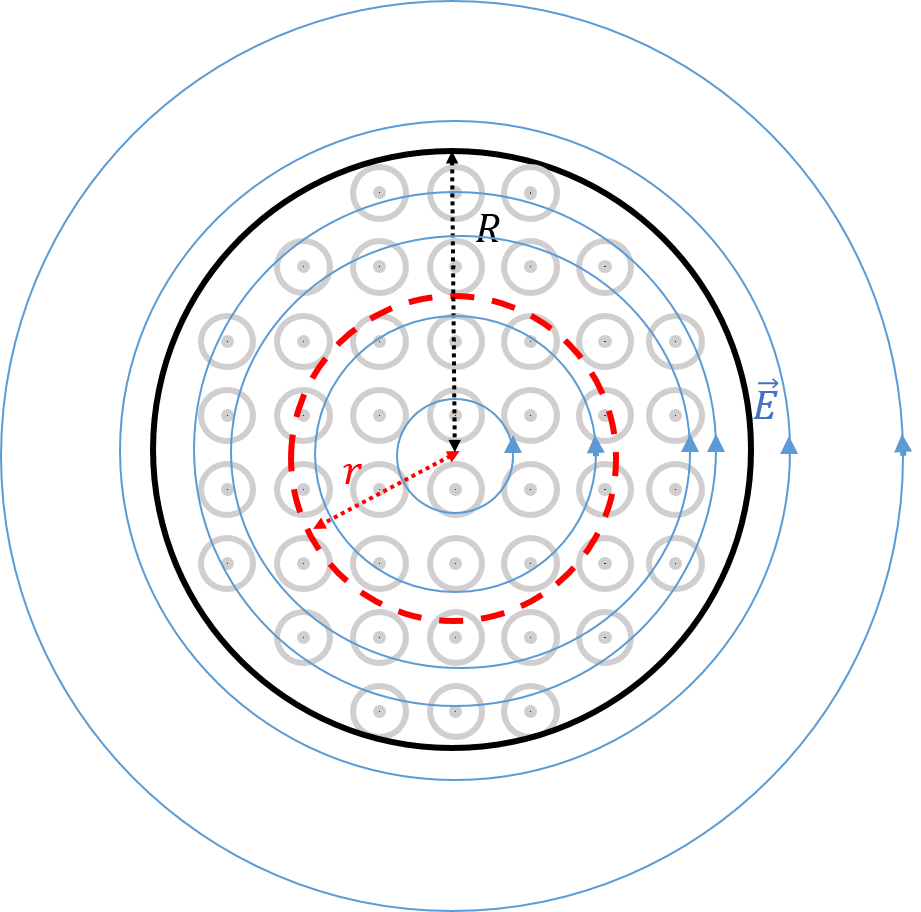
\includegraphics[width=0.4\linewidth]{files/inducedE2-d4dcf4f817ea58569abf12bbaa5f7727.png}
\caption[]{The induced electric field lines form closed circles when the magnetic field changes.}
\label{fig:induction:inducedE2}
\end{figure}

First, we consider the induced electric field in the region with a magnetic field, where $r<R$. We choose a circle of radius $r$ to calculate the flux of the magnetic field. Since the magnetic field is uniform within that region, the flux is given by:
\begin{equation}
\Phi_B = \vec B \cdot \vec A = BA = B_0(1-at) \pi r^2
\end{equation}
The circulation of the electric field is easily found, since the electric field forms concentric circles (by symmetry):
\begin{equation}
\oint \vec E \cdot d\vec l = \oint Edl = E \oint dl = E(2\pi r)
\end{equation}
Applying Faraday's law, the electric field is found to be:
\begin{equation}
\oint \vec E\cdot d\vec l &= -\frac{d\Phi_B}{dt}\\
E(2\pi r) &= -\frac{d}{dt} B_0(1-at) \pi r^2\\
2E &=  B_0ar\\
\therefore E&=\frac{B_0a}{2}r\quad\text{(inside the region of magnetic field)}
\end{equation}
and we see that, inside the region with the magnetic field, the strength of the induced electric field is proportional to the distance from the centre of the region (i.e. it increases linearly with $r$).

For the region where the magnetic field is zero, we again calculate the circulation of the electric field around a circular loop of radius $r>R$:
\begin{equation}
\oint \vec E \cdot d\vec l = \oint Edl = E \oint dl = E(2\pi r)
\end{equation}
The flux of the magnetic field through that loop is however related to the area of the region with the magnetic field (of radius, $R$):
\begin{equation}
\Phi_B = \vec B \cdot \vec A = BA = B_0(1-at) \pi R^2
\end{equation}
Again, applying Faraday's law:
\begin{equation}
\oint \vec E\cdot d\vec l &= -\frac{d\Phi_B}{dt}\\
E(2\pi r) &= -\frac{d}{dt} B_0(1-at) \pi R^2\\
2Er&=  B_0aR^2\\
\therefore E&=\frac{B_0aR^2}{2r}\quad\text{(outside the region of magnetic field)}
\end{equation}
Outside the region with a magnetic field, the magnitude of the electric field decreases with the distance from the centre of the region.

\textbf{Discussion:} In this example, we determined the electric field that is induced by a varying magnetic field. In this case, the electric field lines form closed circles and result in a non-conservative force. When the electric field is formed by a distribution of electric charges, the field lines begin and end on charges, which is not the case for an induced electric field.
\end{framed}
\end{framed}

\begin{framed}
\textbf{Olivia's Thoughts}\\
You'll notice that this version of Faraday's law has a very similar structure to Ampère 's law. Recall that Ampere's law states:
\begin{equation}
\oint \vec B \cdot d\vec l = \mu_0I^{enc}
\end{equation}
The difference is that now we have the circulation of the electric field rather than the magnetic field and instead of the enclosed current we are dealing with the rate of change of the enclosed flux. This is why, in the last example, we used an almost identical process to how we use Ampère 's law.
\end{framed}

\paragraph{Magnetic braking}

When a conducting material moves into a region of magnetic field, an electric field forming closed loops is induced in the material, thus inducing small current loops, called ``eddy currents''. The magnetic field can then exert a force on those currents, effectively resulting in a force on the material. This is the principle behind magnetic braking, which is used in some trains and in other applications.

Figure~\ref{fig:induction:magneticbrake} illustrates how a magnetic brake can be used to slow a rotating wheel made of a conducting material (the material must conduct or the induced electric field will not produce any current). A magnetic field is produced (e.g. by a fixed permanent magnet) in a direction perpendicular to the wheel, over a small area (shown at the bottom of the wheel in Figure~\ref{fig:induction:magneticbrake}).

\begin{figure}[!htbp]
\centering
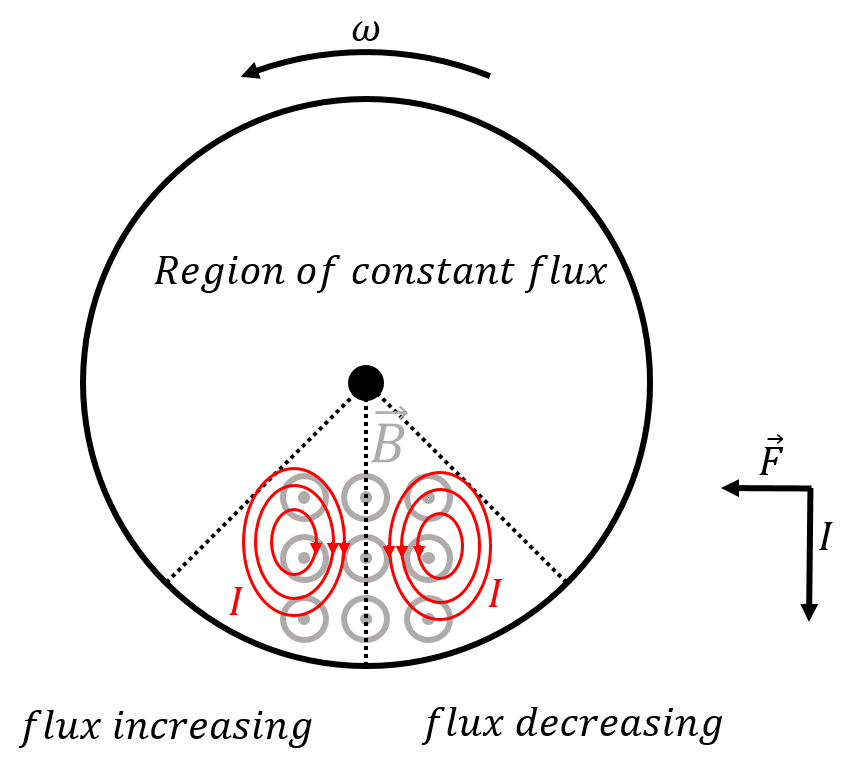
\includegraphics[width=0.6\linewidth]{files/magneticbrake-912a80c2e0d665014177fc2883ff92a1.png}
\caption[]{A rotating wheel made of a conducting material has a small region with a magnetic field. The eddy currents in the region of changing flux result in a net downwards current at the centre of the region. The magnetic force that is exerted on that current slows down the wheel.}
\label{fig:induction:magneticbrake}
\end{figure}

For material located at the bottom left of the wheel, the magnetic flux is increasing, since the material is moving from a region with no magnetic field into a region with a magnetic field. In that part of the region, clockwise eddy currents will form, as those result in a magnetic field into the page, to counter the increasing magnetic flux (Lenz's law). The bottom right side of the wheel is leaving the magnetic field, and will thus have eddy currents in the opposite direction. The currents from both sides add up in the centre, resulting in a net downwards current. The magnetic force on that downwards current is to the left, resulting in a torque that slows the wheel. This is magnetic braking.

Again, this is no more than conservation of energy at play. Since we induce currents by making the wheel move into/out of a region of magnetic field, the electrical energy in those currents must come from somewhere (either we do work to keep the wheel rotating, or the wheel loses kinetic energy). Any time that we try to move a conductor through a magnetic field, in a way that current is induced, we will have to exert a force and do work. In the case of magnetic braking, the wheel will convert its rotational kinetic energy into heat (the eddy currents will heat up the wheel). The main issue with magnetic braking is that one needs to be able to dissipate the heat. The main advantage is that there are no parts that wear out, as opposed to braking with friction. In addition, magnetic braking is very smooth, and only acts when there is motion. As soon as the wheel stops rotating, the magnetic flux is constant everywhere and the eddy currents disappear.

\begin{framed}
\textbf{Checkpoint}\\
Suppose that the magnetic field in Figure~\ref{fig:induction:magneticbrake} pointed into the page. Would the magnetic break still work?

\begin{enumerate}
\item Yes.
\item No.
\end{enumerate}

\begin{framed}
\textbf{Answer}\\
\begin{enumerate}
\item
\end{enumerate}
\end{framed}
\end{framed}

\subsubsection{Transformers}

The electric power generated in power stations is transmitted using high-voltage transmission lines, typically with voltages above $300000 {\rm V}$ for long distances. However, that voltage is not usable in our households, as our appliances expect a voltage around $120 {\rm V}$ (or $220 {\rm V}$ in Europe). Transformers use electromagnetic induction to transform one \textbf{alternating voltage} into another. Figure~\ref{fig:induction:transformer} illustrates a transformer.

\begin{figure}[!htbp]
\centering
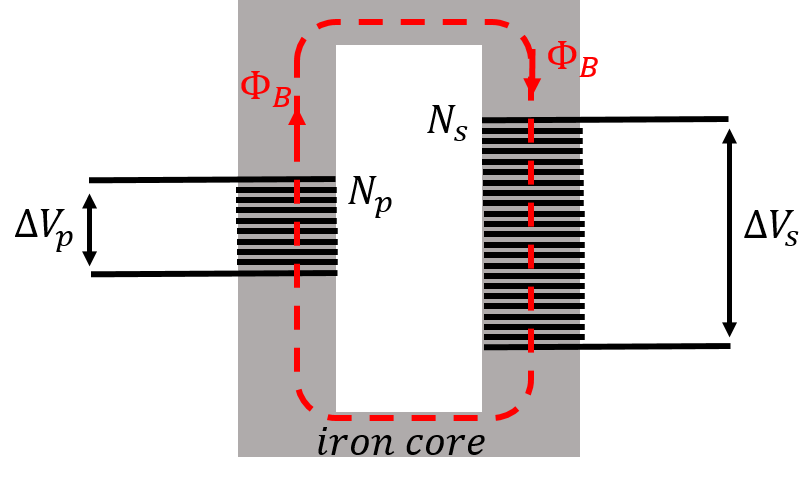
\includegraphics[width=0.5\linewidth]{files/transformer-bcf11362c9aec157a40b39b5e34827ca.png}
\caption[]{A transformer converts a primary alternating voltage, $\Delta V_p$, to a secondary alternating voltage, $\Delta V_s$. The magnetic flux produced in one coil is transmitted by an iron core to the secondary coil, where a different voltage is induced, depending on the ratio of the number of windings in each coil.}
\label{fig:induction:transformer}
\end{figure}

The transformer has two coils, the ``primary'' and the ``secondary'', with different numbers of loops, $N_p$ and $N_s$, respectively. The coils are wrapped around an iron core, which can transmit the magnetic flux generated in the primary coil to the secondary coil. In the transformer, an alternating voltage, $\Delta V_p$, is applied to the primary coil, and transformed into the desired voltage, $\Delta V_s$, in the secondary coil.

The current in the primary coil creates a magnetic field. Those field lines are transmitted by the iron core into the second coil. A voltage is only induced in the secondary coil if the magnetic flux through the secondary coil changes with time. Thus, transformers only work with alternating voltages, so that the magnetic field created by the primary coil changes continuously. Both coils will have the same magnetic flux, $\Phi_B$, through them, since they have the same area. The voltage in the primary coil is given by Faraday's law:
\begin{equation}
\Delta V_p = N_p \frac{d\Phi_B}{dt}
\end{equation}
as is the voltage in the secondary coil:
\begin{equation}
\Delta V_s = N_s \frac{d\Phi_B}{dt}
\end{equation}
Since the flux (and thus its time-derivative) are the same in both coils, we can isolate the time-derivative in each equation to obtain the relationship between the voltages in the two coils:
\begin{equation}
\frac{\Delta V_p}{N_p}&=\frac{\Delta V_s}{N_s}\\
\therefore \Delta V_s &= \frac{N_s}{N_p}\Delta V_p
\end{equation}
Thus, with a transformer, one simply needs to set the ratio of the number of loops in each coil in order to transform one voltage into another.

\begin{framed}
\textbf{Checkpoint}\\
Which coil in Figure~\ref{fig:induction:transformer} has the highest voltage?

\begin{enumerate}
\item The one with the most loops.
\item The one with the least loops.
\end{enumerate}

\begin{framed}
\textbf{Answer}\\
\begin{enumerate}
\item
\end{enumerate}
\end{framed}
\end{framed}

\begin{framed}
\textbf{Checkpoint}\\
Which coil in Figure~\ref{fig:induction:transformer} will have the highest current?

\begin{enumerate}
\item The one with the most loops.
\item The one with the least loops.
\item Not enough information to tell.
\end{enumerate}

\begin{framed}
\textbf{Answer}\\
\begin{enumerate}[resume]
\item
\end{enumerate}
\end{framed}
\end{framed}

\begin{framed}
\textbf{Example 22.3}\\
A power plant produces energy at rate of $P=150 {\rm kW}$, and wishes to transmit this power as efficiently as possible to a town. The power lines between the power plant and the town have a resistance of $R=0.5 {\rm \Omega}$. Compare the amount of power dissipated in the transmission lines depending on whether the power is transmitted through a voltage of $300000 {\rm V}$ or $300 {\rm V}$.

\begin{framed}
\textbf{Solution}\\
We model the transmission of power from the power plant to the town using the circuit shown in Figure~\ref{fig:induction:powerplant}.

\begin{figure}[!htbp]
\centering
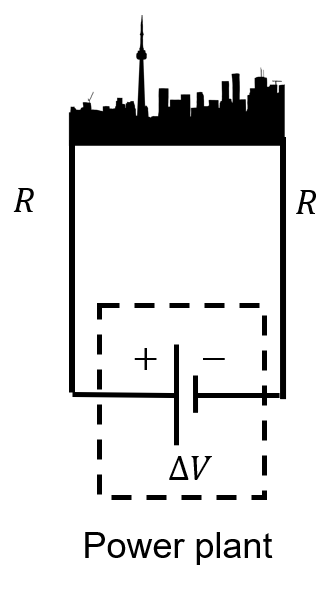
\includegraphics[width=0.25\linewidth]{files/powerplant-b4ec4cc447657225fc944a1bd4e3ab72.png}
\caption[]{Circuit for a power plant transmitting power to a town.}
\label{fig:induction:powerplant}
\end{figure}

We do not know the resistance of the town, but we can still calculate the power that is dissipated in the transmission lines that have a total resistance of $R=0.5 {\rm \Omega}$. The power plant produces power, $P$, and transmits it through the lines at a potential difference, $\Delta V$, resulting in a current, $I$:
\begin{equation}
P &= I\Delta V\\
\therefore I &= \frac{P}{\Delta V}
\end{equation}
The current, $I$, will dissipate power in the lines at a rate of:
\begin{equation}
P_{line} = I^2 R = \frac{P^2}{\Delta V^2}R
\end{equation}
With the two different voltages, this corresponds to:
\begin{equation}
P_{line}&=\frac{P^2}{\Delta V^2}R=\frac{(150e3 {\rm W})^2}{(300000 {\rm V})^2}(0.5 {\rm \Omega})=0.1 {\rm W}\\
P_{line}&=\frac{P^2}{\Delta V^2}R=\frac{(150e3 {\rm W})^2}{(300 {\rm V})^2}(0.5 {\rm \Omega})=125000 {\rm W}\\
\end{equation}
Thus, when the power is transmitted at low voltage, more than 80\% is dissipated in the transmission lines, whereas an insignificant fraction is dissipated when the power is transmitted at high voltage. This is why we need transformers.
\end{framed}
\end{framed}

\subsubsection{Maxwell's equations and electromagnetic waves}

This section is meant to be informative, as the material is beyond the scope of this textbook. Nonetheless, it is worth summarizing what we have learned about electricity and magnetism, as Maxwell did. We can summarize the main laws from electromagnetism as follows:
\begin{equation}
\oint \vec E\cdot d\vec A &= \frac{Q}{\epsilon_0}&\text{(Gauss' Law)}\\
\oint \vec B\cdot d\vec A &= 0 &\text{(No magnetic monopoles)}\\
\oint \vec B\cdot d\vec l &= \mu_0 I^{enc} &\text{(Ampère's Law)}\\
\oint \vec E\cdot d\vec l &= -\frac{d}{dt}\int \vec B\cdot d\vec A  &\text{(Faraday's law)}\\
\end{equation}
where we wrote the magnetic flux in Faraday's law using the integral explicitly. As you recall, Gauss' Law is equivalent to Coulomb's Law, relating the electric field to electric charges that produce the electric field. Although we did not explicitly use the second equation, it is the equivalent to Gauss' Law for the magnetic field. The flux of the magnetic field out of a closed surface must always be zero, since there are no magnetic monopoles, so that magnetic field lines never end.

When we covered Ampère's Law, we only considered a static current as the source of the magnetic field. However, if there is an electric field present that is created by charges that are moving, then those can also contribute a current to Ampère's Law:
\begin{equation}
\oint \vec E\cdot d\vec A &= \frac{Q}{\epsilon_0}\quad \text{(Gauss' Law)}\\
\therefore Q &= \epsilon_0 \oint \vec E\cdot d\vec A\\
\therefore I &= \frac{dQ}{dt} = \epsilon_0\frac{d}{dt} \oint \vec E\cdot d\vec A\\
\end{equation}
so that Ampère's Law, in its most general form, is written:
\begin{equation}
\oint \vec B\cdot d\vec l &= \mu_0 \left(I^{enc}+\epsilon_0\frac{d}{dt} \oint \vec E\cdot d\vec A\right)\quad \text{(Ampère's Law)}
\end{equation}
Writing out the four equations again:
\begin{equation}
\oint \vec E\cdot d\vec A &= \frac{Q}{\epsilon_0} &\text{(Gauss' Law)}\\
\oint \vec B\cdot d\vec A &= 0 &\text{(No magnetic monopoles)}\\
\oint \vec B\cdot d\vec l &= \mu_0 \left(I^{enc}+\epsilon_0\frac{d}{dt} \oint \vec E\cdot d\vec A\right) &\text{(Ampère's Law)}\\
\oint \vec E\cdot d\vec l &= -\frac{d}{dt}\int \vec B\cdot d\vec A  &\text{(Faraday's law)}\\
\end{equation}
These four equations are known as Maxwell's equations, and form our most complete theory of classical electromagnetism. It is quite interesting to note the similarities and relations between the electric and magnetic field. Maxwell's equations contain equations for the circulation and the total flux out of a closed surface for both fields. Ampère's Law implies that a changing electric field will produce a magnetic field. Faraday's law implies that a changing magnetic field produces an electric field. If a point charge oscillates up and down, it will produce a changing electric field, which will produce a changing magnetic field, which will induce a changing magnetic field, etc. This is precisely what an electromagnetic wave is! The light that we see, the Wi-Fi signals for our phones, and the highly penetrating radiation from nuclear reactors are all examples of electromagnetic waves (of different wavelengths).

In fact, as Maxwell did, we can obtain the wave equation (Section~\ref{sec:waves:waveequation}) from Maxwell's equations. We sketch out the derivation here, but it is definitely beyond the scope of this textbook. However, you're so close to seeing one of the most exciting revelations of physics that it would be a shame to skip it!

We first write out Maxwell's equations in differential form, as we have already shown for Gauss' Law ((Section~\ref{sec:gauss:interpretation}) and Ampère's Law ((Section~\ref{sec:magneticsource:interpretation})
\begin{equation}
 \nabla \cdot \vec E &= \frac{\rho}{\epsilon_0} &\text{(Gauss' Law)}\\
 \nabla \cdot \vec B&= 0 &\text{(No magnetic monopoles)}\\
 \nabla \times \vec B &= \mu_0 \left(\vec j + \epsilon_0\frac{\partial\vec E}{\partial t}\right) &\text{(Ampère's Law)}\\
 \nabla \times \vec E &= -\frac{\partial\vec B}{\partial t} &\text{(Faraday's law)}\\
\end{equation}
If we consider a vacuum region in space, with no charges and no currents, these equations reduce to:
\begin{equation}
\nabla \cdot \vec E &= 0 ~~~~&\nabla \cdot \vec B&= 0\\
\nabla \times \vec B &= \mu_0 \epsilon_0\frac{\partial\vec E}{\partial t} ~~~~& \nabla \times \vec E &= -\frac{\partial\vec B}{\partial t}
\end{equation}
We will make use of the following identity from vector calculus:
\begin{equation}
\nabla \times (\nabla \times \vec E)=\nabla(\nabla\cdot \vec E)-\nabla^2\vec E
\end{equation}
where:
\begin{equation}
\nabla^2\vec E &= \frac{\partial^2 \vec E}{\partial x^2}+\frac{\partial^2 \vec E}{\partial y^2} + \frac{\partial^2 \vec E}{\partial z^2}\\
&=\left(\frac{\partial^2 E_x}{\partial x^2}+\frac{\partial^2  E_x}{\partial y^2} + \frac{\partial^2 E_x}{\partial z^2} \right) \hat x+ \left( \frac{\partial^2 E_y}{\partial x^2}+\frac{\partial^2  E_y}{\partial y^2} + \frac{\partial^2 E_y}{\partial z^2} \right) \hat y \\
&+ \left(\frac{\partial^2 E_z}{\partial x^2}+\frac{\partial^2  E_z}{\partial y^2} + \frac{\partial^2 E_z}{\partial z^2}  \right) \hat z
\end{equation}
is called the ``vector Laplacian''.

Consider taking the curl ($\nabla \times$) of the equation that has the curl of the electric field (Faraday's law):
\begin{equation}
\nabla \times \bigg(\nabla \times \vec E &= -\frac{\partial\vec B}{\partial t}\bigg)\\
\nabla(\nabla\cdot \vec E)-\nabla^2\vec E &= -\nabla \times \frac{\partial\vec B}{\partial t}\\
-\nabla^2\vec E &= - \frac{\partial}{\partial t} \nabla \times \vec B\\
-\nabla^2\vec E &= - \frac{\partial}{\partial t} \mu_0 \epsilon_0\frac{\partial E}{\partial t}\\
-\nabla^2\vec E &= - \mu_0 \epsilon_0\frac{\partial^2\vec E}{\partial t^2}
\end{equation}
where, in the third line, we made use of Gauss' Law ($\nabla \cdot \vec E=0$), and, in the fourth line, Ampère's Law ($\nabla \times \vec B = \mu_0 \epsilon_0\frac{\partial E}{\partial t}$). The last equation that we obtained is a vector equation (the vector Laplacian has three components, as does the time-derivative of $\vec E$ on the right-hand side). Consider the $x$ component of this equation:
\begin{equation}
\frac{\partial^2 E_x}{\partial x^2}+\frac{\partial^2  E_x}{\partial y^2} + \frac{\partial^2 E_x}{\partial z^2}  &= \mu_0 \epsilon_0\frac{\partial^2 E_x}{\partial t^2}
\end{equation}
If we define the quantity:
\begin{equation}
c = \frac{1}{\sqrt{\epsilon_0\mu_0}}
\end{equation}
then, the $x$ component of the equation can be written as:
\begin{equation}
\frac{\partial^2 E_x}{\partial x^2}+\frac{\partial^2  E_x}{\partial y^2} + \frac{\partial^2 E_x}{\partial z^2} &= \frac{1}{c^2}\frac{\partial^2 E_x}{\partial t^2}
\end{equation}
which is exactly the wave equation for the component, $E_x$, of the electric field, propagating with speed $c$, the speed of light! Thus, the speed of light is directly related to the constants $\epsilon_0$ and $\mu_0$. You can write out similar equations for the $y$ and $z$ components of the electric field, and find the similar equations for the magnetic field if you start by taking the curl of Ampère's Law instead of Faraday's law.

We have just shown that electric and magnetic fields can behave as waves, which we now understand to be the waves that are responsible for light, radio waves, gamma rays, infra-red radiation, etc. All of these are types of electromagnetic waves with different frequencies. Although we did not demonstrate this, the electromagnetic waves that propagate are such that the magnetic and electric field vectors are always perpendicular to each other. Electromagnetic waves also carry energy. Thus, a charge that is oscillating (say on a spring) and creating an electromagnetic wave must necessarily be losing energy (or work must be done to keep the charge oscillating with the same amplitude). Finally, it is worth noting that, according to Quantum Mechanics, light (and the other frequencies of radiation), are really carried by particles called ``photons''. Those particles are strange, since their propagation is described by a wave equation.

\subsubsection{Summary}

Faraday's law connects a \textbf{changing} magnetic flux to an induced voltage:
\begin{equation}
\Delta V = -\frac{d\Phi_B}{dt}
\end{equation}
The magnetic flux, $\Phi_B$, is calculated as the flux of the magnetic field through an open surface, $S$:
\begin{equation}
\Phi_B = \int_S \vec B\cdot d\vec A
\end{equation}
The induced voltage, $\Delta V$, is the potential difference that is induced along the closed path (a ``loop'') that bounds the surface, $S$. If a charge, $q$, were to move around that closed path, it would gain (or lose) energy, $q\Delta V$. Note that the potential difference that is induced corresponds to a non-conservative electric force, as a charge can gain/lose energy by moving along a closed path. The induced voltage is often called an induced electromotive force (emf), even if it is a voltage.

The minus sign in Faraday's law is sometime referred to as ``Lenz's law'', since it indicates in which direction the induced voltage will be. It is easiest to think of the closed path as a physical wire (e.g. a loop of wire) through which a current will be induced as a result of the induced voltage. The minus sign is easiest to interpret in terms of the relative direction between the area vector used to define the flux, and the magnetic dipole moment vector, $\vec \mu$, associated with the induced current (which points in the same direction as the magnetic field that is produced by the induced current).

When calculating the flux of the magnetic field, the surface element vector $d\vec A$, must be perpendicular to the surface through which the flux is calculated, which leads to two possible choices. Once a choice is made, and Faraday's law has been applied, the sign of $\Delta V$ will indicate if the magnetic dipole moment of the induced current points in the same direction as $d\vec A$ (positive $\Delta V$) or in the opposite direction (negative $\Delta V$).

If $N$ loops of wire are combined together into a coil, the voltages across each loop sum together, so that the voltage induced across the coil is given by:
\begin{equation}
\Delta V = -N\frac{d\Phi_B}{dt}
\end{equation}

Lenz's law is a statement about conservation of energy. Indeed, the induced current must create a magnetic field that \textbf{opposes} the change in flux, otherwise, the induced current would grow indefinitely. Lenz's law can be summarized as follows:

\begin{itemize}
\item If the magnitude of the magnetic \textbf{flux is increasing} in the loop, then the induced current produces a magnetic field that is in the \textbf{opposite direction} from the original magnetic field.
\item If the magnitude of the magnetic \textbf{flux is decreasing} in the loop, then the induced current produces a magnetic field that is in the \textbf{same direction} as the original magnetic field.
\end{itemize}

A voltage is induced along a closed path any time that the flux of the magnetic field through the corresponding surface changes. The flux can change either because the magnetic field is changing, or because the loop is changing (in size or orientation relative to the magnetic field). In the latter case (changing loop), one speaks of a ``motional emf''. A generator creates a motional emf by rotating a coil (with $N$ loops, each with area, $A$), inside a fixed uniform magnetic field, $\vec B$. The voltage produced by a generator is given by:
\begin{equation}
\Delta V = NAB\omega\sin(\omega t)
\end{equation}
where $\omega$ is the angular speed of the coil. A generator thus produces alternating voltage/current. The current that is induced in the coil of the generator will dissipate energy as it flows through a resistance, $R$. Thus, one must do work in order to keep the generator spinning. The current induced in the coil of the generator will also result in a magnetic moment, and a ``counter torque'' will be exerted on the coil. One must thus exert a torque in order to keep the generator spinning (and the work done by exerting that torque is converted into the electrical energy dissipated in the resistor). The counter torque on the generator is always in the same direction, and has a magnitude:
\begin{equation}
\tau = \frac{NA^2B^2\omega\sin^2(\omega t)}{R}
\end{equation}

When an electric motor is used, a ``back emf'' is induced in the coil of the motor. The back emf is such that it resists the direction of current (Lenz's law), or else the motor would spin infinitely fast. As the motor spins faster, the back emf grows, until it reaches an equilibrium. Motors thus draw a large current when they first start up, since at low speed, they have no back emf.

Since a changing magnetic flux induces a voltage, an electric field is also induced. We can replace the voltage in Faraday's law with the circulation of the electric field to write a more general version of Faraday's law:
\begin{equation}
\oint \vec E\cdot d\vec l &= -\frac{d\Phi_B}{dt}
\end{equation}
The induced electric field forms closed field lines, and is different than the electric field that is produced by static charges, since the latter will have field lines that start and end on charges. The force associated with the induced electric field is not conservative.

When a metallic object passes through a region of magnetic field, the induced electric field will induce current loops in the material called eddy currents. The magnetic field will also exert a force on these eddy currents to oppose the motion that is creating the currents (Lenz's law); as the eddy currents dissipate electrical energy in the material, the metallic object must lose kinetic energy unless a force is acting on it. Magnetic brakes make use of this principle.

Transformers are used to convert an alternating voltage, $\Delta V_p$, into a different alternating voltage, $\Delta V_s$. A ``primary'' coil, with $N_p$ windings, creates a changing magnetic flux that is guided (e.g. by an iron core) to a ``secondary'' coil, with $N_s$ windings. The voltage induced in the secondary coil is given by:
\begin{equation}
\Delta V_s &= \frac{N_p}{N_s}\Delta V_p
\end{equation}

Maxwell's four equations form our best classical theory of electromagnetism. Those equations imply that a changing magnetic field produces an electric field (Faraday's law), while a changing electric field can produce a magnetic field (Ampère's Law). By combining Maxwell's equation (with some heavy vector calculus), one can show that this leads to the formation of electromagnetic waves, that propagate with a speed, $c$, given by:
\begin{equation}
c = \frac{1}{\sqrt{\epsilon_0\mu_0}}
\end{equation}

\begin{framed}
\textbf{Important Equations}\\
\textbf{Magnetic flux:}
\begin{equation}
\Phi_B = \int_S \vec B\cdot d\vec A
\end{equation}

\textbf{Faraday's law:}
\begin{equation}
\Delta V = -N\frac{d\Phi_B}{dt}
\end{equation}

\textbf{Faraday's law:}
\begin{equation}
\oint \vec E\cdot d\vec l &= -\frac{d\Phi_B}{dt}
\end{equation}

\textbf{Voltage produced by a generator:}
\begin{equation}
\Delta V = NAB\omega\sin(\omega t)
\end{equation}

\textbf{Counter torque on a generator:}
\begin{equation}
\tau = \frac{NA^2B^2\omega\sin^2(\omega t)}{R}
\end{equation}

\textbf{Secondary voltage in a transformer:}
\begin{equation}
\Delta V_s &= \frac{N_p}{N_s}\Delta V_p
\end{equation}
\end{framed}

\subsubsection{Thinking about the material}

\begin{framed}
\textbf{Reflect and research}\\
\begin{itemize}
\item Who first discovered induction? Why is it called Faraday's law?
\item Give a few examples of applications of magnetic braking.
\item How does a microphone make use of electromagnetic induction?
\item What is magnetic damping?
\item How does an induction stove work?
\item How does a credit card swipe reader make use of induction?
\item What is the origin of Maxwell's equations? When did he publish them?
\item Who was the first to detect electromagnetic waves? How were they produced and detected?
\end{itemize}
\end{framed}

\begin{framed}
\textbf{To try at home}\\
\begin{itemize}
\item Demonstrate magnetic braking by moving a conducting piece of material through a magnetic field.
\end{itemize}
\end{framed}

\begin{framed}
\textbf{To try in the lab}\\
\begin{itemize}
\item Construct an AC generator.
\item Propose an experiment to measure Earth's magnetic field using induction.
\item Propose an experiment to measure a bar magnet's strength using induction.
\end{itemize}
\end{framed}

\subsubsection{Sample problems and solutions}

\paragraph{Problems}

\begin{framed}
\textbf{Problem 22.1}\\
In the 1950s, the Royal Canadian Air Force developed a jet airplane called the Avro Arrow. This jet reached a speed of Mach 1.9 ($652 {\rm ms^{ -1}}$), and was considered one of the most advanced airplanes that existed at the time. Suppose that the Avro Arrow is travelling at a velocity of $v = 652 {\rm ms^{ -1}}$ above the South Pole through Earth's vertical magnetic field, $B = 5.2e -5 {\rm T}$, as shown in Figure~\ref{fig:induction:avro}. If the Avro Arrow had a wingspan of $l = 15 {\rm m}$, determine the induced voltage across its wings.

\begin{figure}[!htbp]
\centering
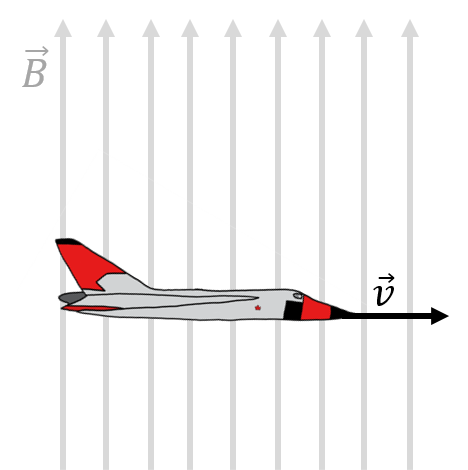
\includegraphics[width=0.25\linewidth]{files/avro-2bee885122f39a9c5de989faa5ab7a4b.png}
\caption[]{The Avro Arrow moving through a magnetic field.}
\label{fig:induction:avro}
\end{figure}
\end{framed}

\begin{framed}
\textbf{Problem 22.2}\\
A generator is made of $N$ circular loops of radius $R=0.3 {\rm m}$, rotating at a frequency of $f=60 {\rm Hz}$ in a uniform magnetic field, $B=0.1 {\rm T}$. How many coils must the generator have in order for it to produce an alternating voltage with a maximum amplitude of $\Delta V =110 {\rm V}$.
\end{framed}

\paragraph{Solutions}

\begin{framed}
\textbf{Solution 22.1}\\
This is identical to the motional emf that is generated by a bar moving in a magnetic field. As the airplane moves as illustrated (towards the left, in an upwards magnetic field), the electrons in the wing of the airplane will be pushed into the page. Eventually, the electric field from the electrons will prevent further electrons from accumulating at that side of the wing, and there will be a constant (Hall) voltage, $\Delta V$, across the wing tips. This will happen when the magnetic and electric force are equal and opposite:
\begin{equation}
qvB &= qE = q\frac{\Delta V}{L}
\end{equation}
where $L$ is the wingspan of the airplane. The induced potential is thus given by:
\begin{equation}
\Delta V = BLv = (5.2e-5 {\rm T})(15 {\rm m})(652 {\rm ms^{-1}})=0.51 {\rm V}
\end{equation}
\end{framed}

\begin{framed}
\textbf{Solution 22.2}\\
The voltage produced by a generator is given by:
\begin{equation}
\Delta V&=NAB\omega\sin(\omega t)
\end{equation}
and the angular frequency is given by $\omega = 2\pi f$. The number of required coils is thus:
\begin{equation}
N=\frac{\Delta V}{AB\omega}=\frac{\Delta V}{\pi R^2B2\pi f}=\frac{(110 {\rm V})}{2\pi^2(0.3 {\rm m})^2(0.1 {\rm T})(60 {\rm Hz})}=10.3
\end{equation}
Thus, one requires 10 loops in the coil to generate the desired voltage.
\end{framed}